\documentclass{article}
\usepackage[dvips]{graphicx}
\usepackage{makeidx}
\usepackage{rotating}
\usepackage{longtable}
\makeindex

\author{Princed Development Team}
\title{Prince~of~Persia\\ Specifications of\\ File Formats}

\begin{document}

\maketitle
\tableofcontents
\newpage

\section{Preamble}

 This file was written thanks to the hard work on reverse engineering made
 by several people, see the credits section. In case you find any mistake
 in the text please report it. A copy of this document should be available
 in our official site at {\it http://www.princed.org}.


\section{Introduction}

 There are two versions of the \index{DAT} DAT file format: DAT v1.0 used in POP 1.x
 and DAT v2.0 used in POP 2. In this document we will specify DAT v1.0.

 DAT files were made to store levels, images, palettes, wave, midi and
 internal speaker sounds. Each type has its own format as described below
 in the following sections.

 As the format is very old and the original game was distributed in disks,
 it is normal to think that the file format uses some kind of checksum
 validation to detect file corruptions.

 DAT files are indexed, this means that there is an index and you can
 access each resource through an ID that is unique for the resource inside
 the file.

 Images store their height and width but not their palette, so the palette
 is another resource and must be shared by a group of images.

 PLV files use the extension defined to support a format with only one
 level inside.

 Both versions of DAT are supported and may be manipulated by \index{PR} PR. This
 program works like an archive manager (i.e. pkzip) and extracts the files
 in known formats that may be handled by other programs. For more
 information about PR check the Princed home page at
 {\it http://www.princed.org}.

 In this document you will also find the \index{SAV} SAV and \index{HOF} HOF format specifications
 and the algorithm used by POP1 to draw the \index{dungeon!walls} dungeon walls.


\section{DAT v1.0 Format Specifications}

\subsection{General file specifications}
 All DAT files have an index, this index has one entry per item with information on each one.

 The index is stored at the very end of the file. But may be located reading the first 6 bytes (as headers) of the file,
 that are reserved to locate the index and know it's size. The sum of the location and the index size should be the size of the file.
 
\subsubsection{Some definitions}

 Let's define the numbers as:
\begin{description}
\item[SC]{ Signed char: 8 bits, the first bit is for the sign and the 7 last
       for the number. If the first bit is a 0, then the number is
       positive, if not the number is negative, in that case invert all
       bits and add 1 to get the positive number.\\
       i.e. -1 is FF (1111 1111), 1 is 01 (0000 0001)\\
       Range: -128 to 127\\
       1 byte}
\item[UC]{Unsigned char: 8 bits that represent the number.\\
       i.e. 32 is 20 (0010 0000)\\
       Range: 0 to 255\\
       1 byte}
\item[US]{Unsigned Short: \index{Little endian} Little endian, 16 bits, storing two groups of 8 bits
       ordered from the less representative to the most representative
       without sign.\\
       i.e. 65534 is FFFE in hex and is stored FE FF (1111 1110  1111 1111)\\
       Range: 0 to 65535\\
       2 bytes}
\item[SS]{Signed Short: Little endian, 16 bits, storing two groups of 8 bits
       ordered from the less representative to the most representative with
       sign. If the first byte is 0 then the number is positive, if not the
       number is negative, in that case invert all bits and add 1 to get
       the positive number.\\
       i.e. -2 is FFFE in hex and is stored FE FF (1111 1110  1111 1111)\\
       Range: -32768 to 32767\\
       2 bytes}
\item[UL]{Unsigned long: Little endian, 32 bits, storing four groups of 8 bits
       each ordered from the less representative to the most representative
       without sign.\\
       i.e. 65538 is 00010002 in hex and is stored 02 00 01 00\\
       (0000 0010  0000 0000  0000 0001  0000 0000)\\
       Range: $0$ to $2^{32}-1$\\
       4 bytes}

\end{description}

 Sizes will always be expressed in bytes unless another unit is specified.\\

\subsubsection{Index structures}

\newcommand{\tableline}[5]{ {\tiny $#1$} & {\tiny $#2$ } & {\tiny #3} & {\tiny $#4$} & {\small #5} \\}
\newcommand{\tablenote}[1]{
 \multicolumn{5}{p{11.7cm}}{ #1 } \\
 \endlastfoot
}
\newcommand{\offsettable}[4]{
 \renewcommand{\tabcolsep}{0.3em}
 \begin{longtable}{ccccp{4cm}}
  \hline
  Offset & Size & Type & Name & Description \\
  \hline
 \endfirsthead
  #1
  \hline
  Offset & Size & Type & Name & Description \\
  \hline
 \endhead
  \hline
  #2
  \hline
 \caption{#3}
 \label{#4}
 \end{longtable}
}

\newcommand{\offsettablee}[4]{
 \renewcommand{\tabcolsep}{1em}
 \begin{longtable}{ccl}
  \hline
  Length& Offset & Block Name \\
  \hline
 \endfirsthead
  #1
  \hline
  Length& Offset & Block Name \\
  \hline
 \endhead
  \hline
  #2
  \hline
 \caption{#3}
 \label{#4}
 \end{longtable}
}

%offset table

\offsettable{
 \tablenote{
  Note: POP1 doesn't validate the DAT file checking $IndexOffset+IndexSize=FileSize$, this means you can append data at the end of the file.
 }
}{
\tableline{0}{4}{UL}{IndexOffset}{The location where the index begins }
\tableline{4}{2}{US}{IndexSize\footnote[1]{$IndexOffset+IndexSize=file size$} }{The number of bytes the index has }
\hline
\hline
\tableline{IndexOffset=\alpha}{IndexSize}{$\downarrow$}{Footer}{The DAT index}
\hline
\tableline{\alpha}{2}{US}{NumberOfItems}{Resources count}
\tableline{\alpha+2=\beta\footnote[2]{so $IndexSize=8*numberOfItems+2$}}{NumberOfItems*8}{-}{Index}{A list of NumberOfItems blocks of 8-bytes-length index record called Entry}
\hline
\hline
\tableline{\beta+8i=\gamma}{8}{$\downarrow$}{Entry}{The 8-bytes-length index record (one per item)}
\hline
\tableline{\gamma+0}{2}{US}{Id(i)\footnote[3]{with $0 \le i < numberOfItems$}    }{Item ID}
\tableline{\gamma+2}{4}{UL}{Offset(i)\footnotemark[3]}{Absolute offset where the resource start}
\tableline{\gamma+6}{2}{US}{Size(i)\footnotemark[3]  }{Size of the item not including the checksum byte}
}{DAT file blocks}{file blocks}

% The \index{DAT} DAT header: Size = 6 bytes
%  - Offset 0, size 4, type UL: IndexOffset
%           (the location where the index begins)
%  - Offset 4, size 2, type US: IndexSize
%           (the number of bytes the index has)
%           Note that $IndexSize$ is $8*numberOfItems+2$
%           Note that $IndexOffset+IndexSize=file size$
%
% The DAT index: Size = IndexSize bytes
%  - Offset $IndexOffset$,   size 2, type US: NumberOfItems
%           (resources count)
%  - Offset $IndexOffset+2$, size $NumberOfItems*8$: The index
%           (a list of NumberOfItems blocks of 8-bytes-length index record)
%
% The 8-bytes-length index record (one per item): Size = 8 bytes
%  - Relative offset 0, size 2, type US: Item ID
%  - Relative offset 2, size 4, type UL: Resource start
%           (absolute offset in file)
%  - Relative offset 6, size 2, type US: Size of the item
%           (not including the checksum byte)

  PR validates that $IndexOffset+IndexSize \le FileSize$.
 It also compares IndexSize with $8*numberOfItems+2$ to determine if a file
  is a valid POP1 DAT file.

\subsubsection{Checksums byte}

 There is a \index{checksum} checksum byte for each item (resource), this is the first byte
 of the item, the rest of the bytes are the item data. The item type is not
 stored and may only be determined by reading the data and applying some
 filters, unfortunately this method may fail. When you extract an item you
 should know what kind of item you are extracting.

 If you add (sum) the whole item data including checksum and take the less
 representative byte (modulus 256) you will get the sum of the file. This
 sum must be FF in hex (255 in UC or -1 in SC). If the sum is not FF, then
 adjust the checksum in order to set this value to the sum. The best way
 to do that is adding all the bytes in the item data (excluding the
 checksum) and inverting all the bits. The resulting byte will be the
 right checksum.

 From now on the specification are special for each data type (that means
 we won't include the checksum byte anymore).

\subsection{Images}
 Images are stored compressed and have a header and a compressed data area.
 Each image only one header with 6 bytes in it as follows

\subsubsection{Headers} %3.2.1

\offsettable{}{
\tableline{0}{6}{$\downarrow$}{ImageHeader}{The header of an image}
\hline
\tableline{0}{2}{US}{Height}{The height of the image in pixels}
\tableline{2}{2}{US}{Width}{The width of the image in pixels}
\tableline{4}{2}{-}{ImageMask}{Information on the compression algorithm and bitrate}
\hline
}{Image headers}{image header blocks}

% The 6-bytes-image header: 6 bytes
%  Relative offset 0, size 2, type US: Height
%  Relative offset 2, size 2, type UL: Width
%  Relative offset 4, size 2: Information

 ImageMask is a set of bits where:
\begin{itemize}
\item[$\diamond$] the first 8 are zeros
\item[$\diamond$] the next 4 are the resolution\\
   so if it is 1011 (B in hex) then the image has 16 colours;
   and if it is 0000 (0 in hex) then the image has 2 colours.
   To calculate the bits per pixel there are in the image, just take the
   last 2 bits and add 1. e. g. 11 is 4 ($2^4=16$ colours) and 00 is 1 ($2^1=2$ colours).
\item[$\diamond$] the last 4 bits are the 5 compression types (from 0 to 4) as specified in Table~\ref{algorithm codes}.
\end{itemize}

\renewcommand{\tabcolsep}{1em}
\begin{longtable}{ccl}
 \hline
  Dec & Bin & Algorithm \\
 \hline
  0 & 0000 & RAW\_LR \\
  1 & 0001 & RLE\_LR \\
  2 & 0010 & RLE\_UD \\
  3 & 0011 & LZG\_LR \\
  4 & 0100 & LZG\_UD \\
 \hline
 \caption{Algorithm codes}
 \label{algorithm codes}
\end{longtable}

 The following data in the resource is the image compressed with the
 algorithm specified by those 4 bits.

\subsubsection{Algorithms} %3.2.2

\begin{description}

\item[RAW\_LR]{means that the data has not been compressed in any way, it is used
        for small images.
        The format is saved from left to right (LR) serialising a line to
        the next integer byte if necessary. In case the image was 16
        colours, two pixels per byte (4bpp) will be used. In case the image
        was 2 colours, 8 pixels per byte (1bpp) will be used.
}
\item[RLE\_LR]{has a \index{Run length encoding|see{RLE}} Run length encoding \index{RLE} (RLE) algorithm, after uncompressed the
        image can be read as a RAW\_LR.}

\item[RLE\_UD]{is the same as RLE\_LR except that after uncompressed the bytes in
        the image must be drawn from up to down and then from left to right.}

\item[LZG\_LR]{ has some kind of variant of the LZ77 algorithm (the sliding windows
        algorithm), here we named it \index{LZG} LZG in honour of Lance Groody, the
        original coder.
        After decompressed it may be handled as RAW\_LR.}
\item[LZG\_UD]{Uses LZG compression but is drawn from top to bottom as RLE\_UD.}

\end{description}

\subsubsection{Run length encoding (RLE)} %3.2.2.1
 The first byte is always a control byte, the format is SC. If the control
 byte is negative, then the next byte must be repeated n times as the bit
 inverted control byte says, after the next byte (the one that was
 repeated) another control byte is stored.\\
 If the control byte is positive or zero just copy textual the next $n$ bytes
 where $n$ is the control byte plus one. After that, the next byte is the
 following control byte.\\
 If you reach a control byte but the image size is passed, then you have
 completed the image.

\subsubsection{LZ variant (LZG)} %3.2.2.2
 This is a simplified algorithm explanation:

 Definition: ``print'' means to commit a byte into the current location
             of the output stream.\\

{\tt
 The output stream is a slide window initialised with zeros.\\
 The first byte of the input stream is a maskbyte.\\
 For each of the 8 bits in the maskbyte the next actions must be performed:\\
  If the bit is 1 print the next unread byte to the slide window\\
  If the bit is a zero read the next two bytes as control bytes with the
  following format (RRRRRRSS SSSSSSSS):\\
\begin{itemize}
\item[$\cdot$] 6  bits for the copy size number ($R$). Add 3 to this number.\\
        Range: $2$ to $2^6+2=66$
\item[$\cdot$] 10 bits for the slide position ($S$). Add 66 to this number.\\
        Range: $2^6+2=66$ to $2^6+2+2^{10}=1090$
\end{itemize}
   Then print in the slide window the next $R$ bytes that are the same slide
   window starting with the $S^{th}$ byte.\\
}
 After all the maskbyte is read and processed, the following input byte is
 another maskbyte. Use the same procedure to finish decompressing the file.
 Remaining unused maskbits should be zeros to validate the file.

 This is the modus operandi of the compression algorithm

 For each input byte we take a window containing the 1023 previous bytes.
 If the window goes out of bounds (ie, when the current input byte is
 before position $2^{10}=1024$), we consider it filled with zeros.

%     00000000000000000000********************************
%                         ^                  ^
%                    input start   current input byte
%           |--------------------------------|
%                    window size=1023
\begin{figure}[h]
\centerline{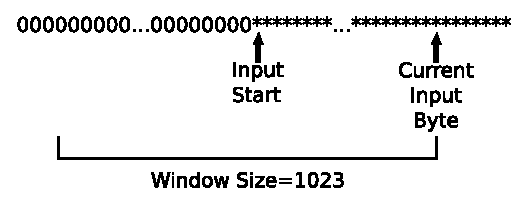
\includegraphics{lzg.eps}}
\caption{Distribution of the sindow size.}
\end{figure}

\pagebreak[2]
 The algorithm works as follows:\\
{\small
\begin{verbatim}
 While there is unread input data:
     Create a maskbyte.
     For each bit in the maskbyte (and there is still unread input data):
         Compare the following input bytes with the bytes in the window,
         and search the longest pattern that is equal to the next bytes.
         If we found a pattern of length n > 2:
             Assign 0 to the current bit of the maskbyte.
             In the next 2 bytes of the output, specify the relative
             position and length of the pattern.
             Advance output pointer by 2.
             Advance input pointer by n.
         Else:
             Assign 1 to the current bit of the maskbyte.
             Copy the current input byte in the next output byte.
             Advance output pointer by 1.
             Advance input pointer by 1.
\end{verbatim}
}
\pagebreak[2]

 For a better understanding of the algorithm we strongly recommend to read
 the \index{PR} \index{LZG} PR source files {\it lzg\_uncompress.c} and {\it lzg\_compress.c} that may be
 located at
 {\fontsize{6}{6}\selectfont {\it https://gforge.lug.fi.uba.ar/plugins/scmcvs/cvsweb.php/PR/src/lib/compression/?cvsroot=freeprince}}
 in the PR repository module.

\pagebreak[3]
\subsection{Palettes}
 Palette resources store a palette for the \index{VGA} VGA and patterns for the \index{CGA} CGA and
 \index{EGA} EGA. Each palette resource is sized 100 bytes distributed as explained in Table~\ref{palettes table}:

\renewcommand{\tabcolsep}{1em}
\begin{longtable}{ccl}
 \hline
  Length & Offset & Block Name \\
 \hline
  4     & 0      & unknown (TGA?) \\
  48    & 4      & vga\_palette \\
  16    & 52     & cga\_patterns \\
  32    & 68     & ega\_patterns \\
 \hline
 \caption{DAT 1.0 Palette blocks}
 \label{palettes table}
\end{longtable}

\pagebreak[2]
 The vga\_palette block stores 16 records of three bytes each that is the
 palette in the RGB-18-bits format (6 bits for each colour). Each colour is
 a number from 0 to 63. Remember to shift the colour bytes by two to get
 the colour number from 0 to 256. The format is 00rrrrrr 00gggggg 00bbbbbb
 where rrrrrr is the 6 bit red, gggggg the 6 bits green and bbbbbb the 6
 bits blue.

\pagebreak[2]
 In the case of EGA and CGA, palettes are not stored. The palettes are the standard ones
 defined by the adapter. In Table~\ref{egacga pals} the standard palettes are shown. 
 
\renewcommand{\tabcolsep}{0.5em}
\begin{longtable}{ccclcc}
 \hline
  EGA & CGA1 & CGA2  & Color name      &  HTML     & rgbRGB \\
 \hline
  0   & 0    & 0     & black           & \verb!#000000!  & 000000 \\
  1   & -    & -     & blue            & \verb!#0000aa!  & 000001 \\
  2   & -    & 1     & green           & \verb!#00aa00!  & 000010 \\
  3   & 1    & -     & cyan            & \verb!#00aaaa!  & 000011 \\
  4   & -    & 2     & red             & \verb!#aa0000!  & 000100 \\
  5   & 2    & -     & magenta         & \verb!#aa00aa!  & 000101 \\
  6   & -    & 3     & brown           & \verb!#aa5500!  & 010100 \\
  7   & 3    & -     & light gray      & \verb!#aaaaaa!  & 000111 \\
  8   & -    & -     & dark gray       & \verb!#555555!  & 111000 \\
  9   & -    & -     & bright blue     & \verb!#5555ff!  & 111001 \\
  10  & -    & -     & bright green    & \verb!#55ff55!  & 111010 \\
  11  & -    & -     & bright cyan     & \verb!#55ffff!  & 111011 \\
  12  & -    & -     & bright red      & \verb!#ff5555!  & 111100 \\
  13  & -    & -     & bright magenta  & \verb!#ff55ff!  & 111101 \\
  14  & -    & -     & bright yellow   & \verb!#ffff55!  & 111110 \\
  15  & -    & -     & bright white    & \verb!#ffffff!  & 111111 \\
 \hline
 \caption{EGA and CGA palettes}
 \label{egacga pals}
\end{longtable}

 Where \index{EGA} EGA is the only one palette used in EGA mode of the game and CGA1
 and CGA2 are the two palettes used in the \index{CGA} CGA mode.
 As the palettes are always the same, but the graphics are in 16 colours,
 some patterns are used instead of colours.
 Remember EGA has 16 colours, so is represented in 4 bits and CGA has 4
 simultaneous colours represented in 2 bits.

\pagebreak[2]
 The cga\_patterns block stores 16 records of one byte each, separated in
 four parts, so the format is $a_0 a_1 b_0 b_1 c_0 c_1 d_0 d_1$ where aa is a two bit colour in one
 of the two CGA palettes (palette 1 is normally used in the \index{dungeon!environment} dungeon
 environment and 2 in the palace environment).
 
 The pattern is arranged in a 2x2 box and each pixel is denoted:
\begin{center}
\begin{tabular}{c|c}
  $a_0 a_1$ & $b_0 b_1$\\
  \hline
  $c_0 c_1$ & $d_0 d_1$\\
\end{tabular}
\end{center}
 
 So for example if the entry 1 is 00101000 (0x28) in mode CGA2, the pattern
 will be a checkerboard of black and green like the following:

\begin{center}
\begin{tabular}{cc|cc|cc}
  \multicolumn{2}{c}{Bin} & \multicolumn{2}{c}{Dec} & \multicolumn{2}{c}{Colour} \\
 \hline
  00 & 01  &    0 & 1 &    black &  green \\
  01 & 00  &    1 & 0 &    green &  black \\
\end{tabular}
\end{center}

 The ega\_patterns block stores 16 records of two bytes each, this time
 separated in two parts. So we have again, four parts per record in the
 format aaaabbbb ccccdddd.
 
 Now, using the EGA entries 0-15 (the four bits are represented) the same
 patterns as the CGA may be used.
 
 For example, with 00101111 11110010 (0x2ff2) you can create the following
 pattern:

\begin{center}
\begin{tabular}{cc|cc|cc|cc}
  \multicolumn{2}{c}{Bin} & \multicolumn{2}{c}{Dec} & \multicolumn{2}{c}{Hex} & \multicolumn{2}{c}{Colour} \\
 \hline
  0010 & 1111  &  2  & 15  & 2 & f &  brown &  white\\
  1111 & 0010  &  15 & 2   & f & 2 &  white &  brown\\
\end{tabular}
\end{center}

\subsection{Levels \label{level blocks}}
 This table has a summary of the blocks to be used in this section,
 you can refer it from the text below.

\pagebreak[3]
\offsettablee{}{
  720   & 0      & pop1\_foretable \\
  720   & 720    & pop1\_backtable \\
\index{foretable}
\index{backtable}
  256   & 1440   & door I \\
  256   & 1696   & door II \\
  96    & 1952   & links \\
  64    & 2048   & unknown I \\
  3     & 2112   & start\_position \\
  3     & 2115   & unknown II \\
  1     & 2116   & unknown III \\
  24    & 2119   & guard\_location \\
  24    & 2143   & guard\_direction \\
  24    & 2167   & unknown IV (a) \\
  24    & 2191   & unknown IV (b) \\
  24    & 2215   & guard\_skill \\
  24    & 2239   & unknown IV (c) \\
  24    & 2263   & guard\_colour \\
  16    & 2287   & unknown IV (d) \\
  2     & 2303   & 0F 09 (2319) \\
}{DAT 1.0 Level blocks}{dat1 level}
\pagebreak[3]

 All levels have a size of 2305, except in the original game, that the
 potion level has a size of 2304 (may be it was wrong trimmed).

\subsubsection{Unknown blocks} %3.4.1
 Blocks described in this section are: Unknown from I to IV.

 Unknown III and IV blocks does not affect the level if changed, if you
 find out what they are used to we will welcome your specification text.

 Unknown I may corrupt the level if edited.

 We believe unknown II has something to do with the start position, but we
 do not know about it.

 As unknown II were all zeros for each level in the original set, it was a
 team decision to use those bytes for format extension. If one of them is
 not the default 00 00 00 hex then the level was extended by the team.
 Those extensions are only supported by RoomShaker at this  moment. To see
 how those extensions were defined read the appendix I will write some day.
 For the moment you may contact us if you need to know that.

\subsubsection{Room mapping\label{room mapping}} %3.4.2
 This section explains how the main walls and objects are stored. The
 blocks involved here are ``pop1\_foretable'' and ``pop1\_backtable''

 In a level you can store a maximum of 24 rooms (also called screens) of 30
 tiles each, having three stages of 10 tiles each. Screens are numbered
 from 1 to 24 (not 0 to 23) because the 0 was reserved for special cases.

 The pop1\_foretable and pop1\_backtable blocks have 24 sub-blocks inside.
 Those sub-blocks have a size of 30 bytes each and has a room associated.
 So, for example, the sub-block staring in 0 corresponds to the room 1 and
 the sub-block starting in 690 corresponds to the room 24.
 It is reserved 1 byte from the pop1\_foretable block and one from the
 pop1\_backtable block for each tile. To locate the appropriate tile you
 have to do the following calculation: $tile=(room-1)*30+tileOffset$ where
 tileOffset is a number from 0 to 29 that means a tile from 0 to 9 if in
 the upper stage, from 10 to 19 if in the middle stage and 20 to 29 if in
 the bottom stage. We define this as the location format and will be used
 also in the start position.
 Always looking from the left to the right.
 So there is a pop1\_foretable and pop1\_backtable byte for each tile in the
 level and this is stored this way.

 The pop1\_foretable part of the tile stores the main tile form according to
 the table below. Note that those are just a limited number of tiles, each
 code has a tile in the game. The tiles listed are all the ones needed to
 make a level so the missing tiles have an equivalent in this list.

 Each tile has a code id, as some codes are repeated this is how you have
 to calculate the codes. A tile in the pop1\_foretable part has 8 bits in
 this format rrmccccc, where rr are random bits and can be ignored. m is a
 modifier of the tile. For example modified loose floors do not fall down.
 The rest ccccc is the code of the tile tabled below. Tile names are the
 same as the ones used by RoomShaker to keep compatibility.

\begin{longtable}{cccl}
\hline
 Hex & Binary& Group & Description \\
\hline
\endfirsthead
\hline
 Hex & Binary& Group & Description \\
\hline
\endhead
0x00 & 00000 & free  & Empty \\
0x01 & 00001 & free  & Floor \\
0x02 & 00010 & spike & Spikes \\
0x03 & 00011 & none  & Pillar \\
0x04 & 00100 & gate  & Gate \\
0x05 & 00101 & none  & Stuck Button \\
0x06 & 00110 & event & Drop Button \\
0x07 & 00111 & tapest& Tapestry \\
0x08 & 01000 & none  & Bottom Big-pillar \\
0x09 & 01001 & none  & Top Big-pillar \\
0x0A & 01010 & potion& Potion \\
0x0B & 01011 & none  & Loose Board \\
0x0C & 01100 & ttop  & Tapestry Top \\
0x0D & 01101 & none  & Mirror \\
0x0E & 01110 & none  & Debris \\
0x0F & 01111 & event & Raise Button \\
0x10 & 10000 & none  & Exit Left \\
0x11 & 10001 & none  & Exit Right \\
0x12 & 10010 & chomp & Chopper \\
0x13 & 10011 & none  & Torch \\
0x14 & 10100 & wall  & Wall \\
0x15 & 10101 & none  & Skeleton \\
0x16 & 10110 & none  & Sword \\
0x17 & 10111 & none  & Balcony Left \\
0x18 & 11000 & none  & Balcony Right \\
0x19 & 11001 & none  & Lattice Pillar \\
0x1A & 11010 & none  & Lattice Support \\
0x1B & 11011 & none  & Small Lattice \\
0x1C & 11100 & none  & Lattice Left \\
0x1D & 11101 & none  & Lattice Right \\
0x1E & 11110 & none  & Torch with Debris \\
0x1F & 11111 & none  & Null \\
\hline
\caption{POP1 Foretable codes}
\label{palettes table}
\end{longtable}

 The pop1\_backtable part of the tile stores a modifier or attribute of the
 pop1\_foretable part of the tile. This works independently of the modifier
 bit in the code. The tile modifier depends on the group the tile belongs
 which are wall, chomp, event, ttop, potion, tapp, gate, spike and free.
 The group event allows the 256 modifiers and will be described in Section~\ref{door events}.
% Note + means allowed for the dungeon environment, - means allowed for the
% palace environment.
 
 In the original game all elements are allowed in all levels, but it is possible to set it up
Hex-editing the uncompressed version. To do that, read the Hex editing documentation.

\begin{longtable}{ccl}

\hline
 Group & Code & Description \\
\hline
\endfirsthead
\hline
 Group & Code & Description \\
\hline
\endhead
\multicolumn{3}{p{8cm}}{
 Note: Some modifiers have not been tested, there may be any other unknown
       tile type we have not still discover.

} \\
\endlastfoot

 none  & 0x00 & This value is used always for this group \\
 free  & 0x00 & Nothing\footnote[1]{Dungeon environment \label{id:de}}, Blue line\footnote[2]{Dungeon environment \label{id:pe}} \\
 free  & 0x01 & Spot1\footnotemark[1], No blue line\footnotemark[2] \\
 free  & 0x03 & Window \\
 free  & 0xFF & Spot3\footnotemark[1], Blue line?\footnotemark[2] \\
 spike & 0x00 & Normal (allows animation) \\
 spike & 0x01 & Barely Out \\
 spike & 0x02 & Half Out \\
 spike & 0x03 & Fully Out \\
 spike & 0x04 & Fully Out \\
 spike & 0x05 & Out? \\
 spike & 0x06 & Out? \\
 spike & 0x07 & Half Out? \\
 spike & 0x08 & Barely Out? \\
 spike & 0x09 & Disabled \\
 gate  & 0x00 & Closed \\
 gate  & 0x01 & Open \\
 tapest & 0x00 & With Lattice\footnotemark[2] \\
 tapest & 0x01 & Alternative Design\footnotemark[2] \\
 tapest & 0x02 & Normal\footnotemark[2] \\
 tapest & 0x03 & Black\footnotemark[2] \\
 potion & 0x00 & Empty \\
 potion & 0x01 & Health point \\
 potion & 0x02 & Life \\
 potion & 0x03 & Feather Fall \\
 potion & 0x04 & Invert \\
 potion & 0x05 & Poison \\
 potion & 0x06 & Open \\
 ttop  & 0x00 & With lattice\footnotemark[2] \\
 ttop  & 0x01 & Alternative design\footnotemark[2] \\
 ttop  & 0x02 & Normal\footnotemark[2] \\
 ttop  & 0x03 & Black\footnotemark[2] \\
 ttop  & 0x04 & Black\footnotemark[2] \\
 ttop  & 0x05 & With alternative design and bottom\footnotemark[2] \\
 ttop  & 0x06 & With bottom\footnotemark[2] \\
 ttop  & 0x07 & With window\footnotemark[2] \\
 chomp & 0x00 & Normal \\
 chomp & 0x01 & Half Open \\
 chomp & 0x02 & Closed \\
 chomp & 0x03 & Partially Open \\
 chomp & 0x04 & Extra Open \\
 chomp & 0x05 & Stuck Open \\
 wall  & 0x00 & Normal\footnotemark[1], Blue line\footnotemark[2] \\
 wall  & 0x01 & Normal\footnotemark[1], No Blue line\footnotemark[2] \\
\hline

\caption{Background modifiers by group}
\label{background modifiers}
\end{longtable}

\subsubsection{Wall drawing algorithm} %\ref{room mapping}.1
 This section does not have a direct relation with the format because it
 describes how the walls must be drawn on the room. However, as this
 information should be useful to recreate a cloned room read from the
 format we decided to include this section to the document.

 Wall drawing depends on what is in the right panel. If the right panel
 is not a wall (binary code ends in 10100) a base wall will be drawn and
 other random seed will be used. If the right panel is a wall then the main
 base wall will be drawn and the described seed will be used.

 When the base wall is drawn, the modifiers should be blitted over it.
 There are 53 different types of walls using the same base image.
 We will call the seed array to the one having the modifier information of
 those 53 panels. This array has indexes from 1 to 53 included.

 To calculate what value take from the array this calculation must be
 performed: $panelInfo=seedArray[roomNumber+wallPosition]$
 where panelInfo is the result modifier information that will be applied to
 the base image; seedArray is this array that will be described above as a
 table; roomNumber is the number of the room the wall is (from 1 to 24)
 and wallPosition is the position the wall is (from 0 to 29), using the
 location format specified in section \ref{room mapping}. This means the first value is
 1 (roomNumber=1 and wallPosition=0) and the last is 53 (roomNumber=24
 and wallPosition=29).

 Modifiers affects the corners of a stone. There are three stone rows per
 wall. If the modifier is activated this corner will appear different
 (seems to be darker). Another modifier is the grey stone.

\renewcommand{\tabcolsep}{1em}
\begin{longtable}{ll}
  \hline
 Modifier      & Seed Positions \\
  \hline
 \endfirsthead
  \hline
 Modifier      & Seed Positions \\
  \hline
 \endhead
 \multicolumn{2}{c}{{\it (First row)}} \\
\hline
 Grey stone    & 2, 5, 14, 17, 26, 32, 35, 50 \\
 Left, bottom  & 2, 11, 36, 45 \\
 Left, top     & 37 \\
 Right, bottom & 27, 33 \\
 Right, up     & 4, 10, 31, 37 \\
 \\
\hline
 \multicolumn{2}{c}{{\it (Second row)}} \\
\hline
 Grey stone    & none  \\
 Left, bottom  & 34, 47 \\
 Left, top     & 9, 10 \\
 Right, bottom & 2, 8, 25, 35 \\
 Right, top    & 6, 12, 23, 29, 39 \\
 \\
\hline
 \multicolumn{2}{c}{{\it (Third row)}} \\
\hline
 Grey stone    & none  \\
 Left, bottom  & none \\
 Left, top     & 16 \\
 Right, bottom & none \\
 Right, top    & none \\
\hline
\caption{Stone modifiers on seed position}
\label{seeds}
\end{longtable}

 Another modifiers are saved in the seed too. Those modifiers are not
 boolean values, they are offsets and sizes. As each stone has a different
 size the stone separation offset is saved in the seed.

 For the first row, the stones are all the same size and the seed is not
 needed.

 For the second row we have got the first 20 values, ordered from 1 to 20. \\ 
\renewcommand{\tabcolsep}{0.1em}
\begin{longtable}{r@{\hspace{1cm}}cccccccccccccccccccc}
  \hline
 Field      & \multicolumn{20}{c}{Values} \\
  \hline
 \endfirsthead
 position  &     1&2&3&4&5&6&7&8&9&10&11&12&13&14&15&16&17&18&19&20 \\
 offsets   &     5&4&3&3&1&5&4&2&1& 1& 5& 3& 2& 1& 5& 4& 3& 2& 5& 4 \\
 separator size& 0&1&1&0&0&0&1&1&0& 0& 1& 1& 1& 0& 0& 1& 1& 1& 0& 0 \\
\hline
\caption{First 20 seed values of the second row separator}
\label{seedss}
\end{longtable}

 We will be adding the next values as soon as we count the pixels ;)
 This information can be found in walls.conf file from FreePrince.

\subsubsection{Room linking \label{room linking}} %3.4.3
 This section describes the links block.

 Each room is linked to another by each of the four sides. Each link
 is stored. There is no room mapping, just room linking.

 The links block has 24 sub-blocks of 4 bytes each. All those sub-blocks
 has its own correspondence with a room (the block starting at 0 is
 related to the room 1 and the block starting at with 92 is related to
 room 24).
 Each block of 4 bytes stores the links this room links to reserving one
 byte per each side in the order left (0), right (1), up (2), down (3).
 The number 0 is used when there is no room there.
 Cross links should be made to allow the kid passing from a room to
 another and then coming back to the same room but it is not a must.

\subsubsection{Guard handling\label{guard handling}} %3.4.4
 This section specifies the blocks: guard\_location, guard\_direction,
 guard\_skill and guard\_colour.\\

 Each guard section has 24 bytes, each byte of them corresponds to a room
 so byte 0 is related to room 1 and byte 23 is related to room 24.
 This room is where the guard is located. The format only allows one
 guard per room. Each block describes a property or attribute of the guard.\\

 The guard\_location part of a guard describes where in the room the guard
 is located, this is a number from 0 to 29 if the guard is in the room or
 30 if there is no guard in this room. Other values are allowed but are
 equivalent to 30. The number from 0 to 29 is in the location format
 specified in Section~\ref{room mapping}.\\

 The guard\_direction part describes where the guard looks at. If the value
 is 0, then the guard looks to the right, if the value is the hex FF (-1 or
 255) then he looks left. This is the direction format, and will be used in
 the start position too.

 The guard\_skill is how the guard fights, style and hit points. Note that
 the hit points also depends on the level you are. Allowed numbers are from
 0 to 9.

% TODO: add a skill table

 The guard\_colour is the palette the guard has (see Section~\ref{binary files}).
 The default colours are in this table:

\renewcommand{\tabcolsep}{1em}
\begin{longtable}{ccc}
\hline
Code & Pants    & Cape \\
\hline
0x00 & Light    & Blue Pink \\
0x01 & Red      & Purple \\
0x02 & Orange   & Yellow \\
0x03 & Green    & Yellow \\
0x04 & Dark Blue& Beige \\
0x05 & Purple   & Beige \\
0x06 & Yellow   & Orange \\
\hline
\caption{Default Guard colours}
\label{palettes table}
\end{longtable}

 Other codes may generate random colours because the game is reading
 the palette from trashed memory. This may also cause a game crash.
 It is possible to add new colours in the guard
 palette resource (see Section~\ref{binary files}) avoiding the crash.

\subsubsection{Start Position \label{start position}} %3.4.5
 This section describes the start\_position block.

 This block stores where and how the kid starts in the level. Note that all
 level doors that are on the starting room will be closed in the moment
 the level starts.

 This block has 3 bytes.
 The first byte is the \index{room} room, allowed values are from 1 to 24.
 The second byte is the \index{location} location, see the section \ref{room mapping} for the location
 format specifications.
 The third byte is the \index{direction} direction, see \ref{guard handling} for the direction format
 specifications.

\subsubsection{Door events\label{door events}} %3.4.6
 This section explains how the doors are handled and specifies the blocks
 door I and II.

 First of all he have to define what an event line is in this file. An
 event line is a link to a door that will be activated. If the event was
 triggered with the action close, then the event will close the door, if
 the action was open then the event will open the door. An event line has
 also a flag to \index{trigger} trigger the next event line or not.
 An event is defined as a list of event lines, from the first to the last.
 The last must have the trigger-next-event-line flag off. This is like a
 list of doors that performs an action.
 An event performs the action that it was called to do: open those doors or
 close them. This action is defined by the type of tile pressed.
 Each event line has an ID from 0 to 255. An event has the ID of the first
 event line in it.

 In section \ref{room mapping} it is explained how a door trigger is associated to an
 event ID. Those are the tiles that starts the event depending on what are
 them: closers or openers.

 How events are stored:
 Each door block has 256 bytes, one per event line. Each event line is
 located in an offset that is the event line ID, so event line 30 is
 located in the byte 30 of each block.
 There is a door I part of an event line and a door II part of it. We will
 define them as byte I and byte II.
 You can find there: the door room, the door location, and the
 trigger-next flag. The format is the following:

 Let's define
  Screen $S = s_1 s_2 s_3 s_4 s_5$ as a 5-bit-number from 1 to 24 (5 bits) where $s_n$ is the bit $n$ of the binary representation and whose value represents the screen \index{room|see{screen}} \index{screen} number;
  Location $L = l_1 l_2 l_3 l_4 l_5$ as another 5-bit-number from 0 to 29 where $l_n$ is the bit $n$ of the binary representation whose value is according to the location format specifications (See Section~\ref{guard handling}) \index{location};
  Trigger-next $T = t_1$ as one bit having 1 for ``off'' or a 0 for ``on''.\\

 Byte I  has the form: $t_1 s_4 s_5 l_1 l_2 l_3 l_4 l_5$ \\
 Byte II has the form: $s_1 s_2 s_3  0  0  0  0  0$ \\

\subsection{Digital Waves}
 Read them as raw digital wave sound using the following specifications:

\renewcommand{\tabcolsep}{0.5em}
\begin{longtable}{rl}
  \hline
  Field&Value\\
  \hline
 \endfirsthead
  \hline
  Field&Value\\
  \hline
 \endhead
  Size of Format& 16 \\
  Format&         PCM \\
  Attributes&     8 bit, mono, unsigned \\
  Channels&       1 \\
  Sample rate&    11025 \\
  Bytes/Second&   11025 \\
  Block Align&    1 \\
\hline
\caption{Wave Specifications}
\label{wave specs}
\end{longtable}

 GNU/Linux users can play the raw waves just dropping them inside /dev/dsp
 As DAT headers are very small it is valid to type in a shell console with
 dsp write access: \verb!cat digisnd?.dat>/dev/dsp! to play the whole wave files.

\subsection{Midi music}
 Standard MIDI files. There have been reports that some versions of MIDI
 did not work, but we believe this can bi fixed saving in other MIDI
 format variant (like type 0).

\subsection{Internal PC Speaker}

\offsettable{}{
0 & 3 & $\downarrow$ & $ Header $ & The file header \\
\hline
0 & 2 & UC & $Junk$ & 0x00 (or 0x80 sometimes) \\
2 & 1 & US & $bps$ & Beats per two seconds \\
\hline
0 & $3 numberOfNotes$ & $\downarrow$ & $Body$ & The file body \\
\hline
$3i$ & 2 & US & $Freq$ & frequency in hertz (0 if no sound, 1 or 2 if marker) \\
$3i+2$ & 1 & US & $length$ & length in beats \\
\hline
0 & 2 & $\downarrow$ & $Footer$ & The file footer \\
\hline
0 & 2 & - &  $Junk$  & 0x12 0x00 \\
}{DAT file blocks}{file blocks}


% Header: 3 bytes
%  First byte: 0x00 (or 0x80 sometimes).
%  Next 2 bytes: how many beats per 2 seconds.

% Body: numberOfNotes*3
%  Then, 3 bytes for each note:
%   - 2 bytes: US for frequency in hertz (0 if no sound, 1 or 2 if marker).
%   - 1 byte:  UC for length in beats.

% Footer: 2 bytes
%  Last 2 bytes: 0x12 0x00.

\subsection{Binary files \label{binary files}}
 Some binary files contains relevant information
 The resource number 10 in prince.dat has the \index{VGA} VGA guard palettes in it
 saving n records of a 16-colour-palette of 3 bytes in the specified
 palette format.

\subsection{Levels in POP1 for Mac}
 In the case of Mac, executable and resource data are embedded in the 
 one run-time file. Level data is a part of resources, for examples
 graphics, icons and sounds. Level blocks are very similar to PC but
 not exactly identical. Following table has a summary of the blocks of
 DAT 1.0 for Mac.
\pagebreak[3]
 
\offsettablee{}{
 720   & 0      & pop1\_foretable \\
 720   & 720    & pop1\_backtable \\
 256   & 1440   & door I \\
 256   & 1696   & door II \\
 96    & 1952   & links \\
 64    & 2048   & unknown I \\
 3     & 2112   & start\_position \\
 21    & 2115   & unknown II+III \\
 24    & 2136   & guard\_location \\
 24    & 2160   & guard\_direction \\
 24    & 2184   & unknown IV (a) \\
 24    & 2208   & unknown IV (b) \\
 24    & 2232   & guard\_skill \\
 24    & 2256   & unknown IV (c) \\
 24    & 2280   & guard\_colour \\
 4     & 2304   & unknown IV (d) \\
}{DAT 1.0 Level blocks for Mac}{mac level blocks}

  All levels have a size of 2308. Also there are two different things 
  in comparison with DAT 1.0 for PC. DAT 1.0 for \index{Mac} Mac does not have 
  any index and checksums. 16 levels including demo and potion level
  are only chained in sequence. See~\ref{level blocks} for reference on each block.

\pagebreak[3]
\section{DAT v2.0 Format Specifications}

\subsection{General file specifications}
 POP2 DAT files are not much different from their POP1 predecessors.
 The format is similar in almost each way. The main difference is in the
 index. As DAT v1.0 used an index in the high data, the DAT v2.0 indexes
 are two level encapsulated inside a high data. So there is an index of
 indexes.

 We will use the same conventions than in the prior chapter.
 The checksum validations are still the same.

\offsettable{}{
0 & 6 & $\downarrow$ & $ Header $ & The file header \\
\hline
0 & 4 & UL & $HighDataOffset$ & The location where the highData begins \\
4 & 2 & US & $HighDataSize$ & the number of bytes the highData has \\
}{High data structures}{hds}

% The DAT header: Size = 6 bytes
%  - Offset 0, size 4, type UL: HighDataOffset
%           (the location where the highData begins)
%  - Offset 4, size 2, type US: HighDataSize
%           (the number of bytes the highData has)
%           Note that $HighDataOffset+HighDataSize=file size$

 This is similar to DAT v1.0 format, except that the index area is now
 called high data.

 The high data part of the file contains multiple encapsulated indexes.
 Each of those index is indexed in a high data index of indexes. We will
 call this index the \index{Index!Master} {\it master index} and the sub index the \index{Index!Slave} {\it slave indexes}.
 Slave indexes are the real file contents index.

\subsubsection{The master index} %4.1.1

\offsettable{}{
\tableline{HighDataOffset}{HighDataSize}{$\downarrow$}{Footer}{The DAT index}
\hline
\tableline{0}{2}{US}{NumberOfSlaveIndexes}{the number of the high data sections}
\tableline{2}{$NumberOfSlaveIndexes*6$}{$\downarrow$}{MIRecords}{The master index
           record (a list of NumberOfSlaveIndexes blocks of 6-bytes-length
           index record each corresponding to one slave index}
\hline
\hline
\tableline{0}{6}{$\downarrow$}{MIRecord}{The DAT index}
\hline
\tableline{0}{4}{text}{SID}{4 ASCII bytes string denoting
           the Slave Index ID. The character order is inverted.}
\tableline{4}{2}{US}{SlaveIndexOffset}{slave index offset relative to $HighDataOffset$}
\hline
\hline
}{DAT 2.0 Master index}{mi}

%  - Offset $HighDataOffset$,   size 2, type US: NumberOfSlaveIndexes
%           (the number of the high data sections)
%  - Offset $HighDataOffset+2$, size $NumberOfSlaveIndexes*6$: The master index
%           record (a list of NumberOfSlaveIndexes blocks of 6-bytes-length
%           index record each corresponding to one slave index)

% The 6-bytes-length index record (one per item): Size = 6 bytes
%  - Relative offset 0, size 4, type sting: 4 ASCII bytes string denoting
%           the Slave Index ID. The character order is inverted.
%  - Relative offset 4, size 2, type US: $SlaveIndexOffset$
%           (slave index offset relative to HighDataOffset)

}{DAT 2.0 Master index}{mi blocks}

 From the end of the \index{Index!Master} DAT High Data Master Index to the end of the file
 we will find the High Data section contents (where the HighDataOffset
 relative offsets points to). This content has a set of second indexes
 each called Slave Index. So, to find a Slave Index offset you have to
 add the file HighDataOffset to the SlaveIndexOffset for the desired
 index.

 There are different 4-byte-length ASCII strings called Slave Index IDs.
 When the string is less than 4 bytes, a tailing byte 0x00 is used. We will
 denote it with the null-space symbol ``\textvisiblespace''. The character order is inverted, so
 for example the text SLAP becomes PALS, MARF becomes FRAM, \textvisiblespace\textvisiblespace\textvisiblespace\textvisiblespace
 \ becomes empty or RCS\textvisiblespace \ becomes SCR. They must be in upper case.

\renewcommand{\tabcolsep}{0.5em}
\begin{longtable}{ccl}
 \hline
 ID    & Stored& Description \\
 \hline
 \endfirsthead
 \hline
 ID    & Stored& Description \\
 \hline
 \endhead
 ``cust''& TSUC  & Custom  \\
 ``font''& TNOF  & Fonts \\
 ``fram''& MARF  & Frames \\
 ``palc''& CLAP  & CGA Palette \\
 ``pals''& SLAP  & SVGA Palette \index{palette} \\
 ``palt''& TLAP  & TGA Palette \\
 ``piec''& CEIP  & Pieces   \\
 ``psl'' & LSP\textvisiblespace  & ?  \\
 ``scr'' & RCS\textvisiblespace  & Screens (images that have the full room) \\
 ``shap''& PAHS  & Shapes (normal graphics) \\
 ``shpl''& LPHS  & Shape palettes \\
 ``strl''& LRTS  & Text \\
 ``snd'' & DNS\textvisiblespace  & Sound \\
 ``seqs''& SQES  & Midi sequences \\
 ``txt4''& 4TXT  & Text \\
 ``''    & \textvisiblespace\textvisiblespace\textvisiblespace\textvisiblespace  & Levels \\
\hline
\caption{Slave Index ID strings}
\label{slave indexes}
\end{longtable}

\subsubsection{The slave indexes \label{slave indexes}} %4.1.2
 All encapsulated sections pointed by the Master Index are Slave Indexes.
 The slave index is specified with:
  - Offset SlaveIndexOffset,   size 2, type US: NumberOfItems
           (the number of the records referring to the file data)
  - Offset SlaveIndexOffset+2, size NumberOfItems*11: The slave index
           record (a list of NumberOfItems blocks of 11-byte-length index
           record each corresponding to one slave index)

 The 11-byte-length slave index record (one per item): Size = 11 bytes
  - Relative offset 0, size 2, type US: Item ID
  - Relative offset 2, size 4, type UL: Resource start
           (absolute offset in file)
  - Relative offset 6, size 2, type US: Size of the item
           (not including the checksum byte)
  - Relative offset 8, size 3, type binary: A flags mask
           (in ``shap'' indexes it is always 0x40 0x00 0x00;
           in others 0x00 0x00 0x00)

%todo

 Finally, we can locate whatever item we want if we have the
 \begin{itemize}
 \item[--] Slave Index ID
 \item[--] Item ID
 \end{itemize}
 this is not a unique key, unfortunately we have found repeated pairs of
 IDs for different items, so we have to use the ``order'' as a third key.

 So, the way to find an item is: first read the High Data Offset, go there,
 read the number of slave items, iterate the master index to find the
 desired slave item comparing it with the Slave Index ID. Then go to the
 found Slave Index offset (remember to add the High Data Offset) and read
 the number of items for this index. Finally iterate the slave index to
 find the desired item comparing the Item ID and read the offset and size.
 Now you will have the offset of the desired item's checksum, increasing
 the offset by one will give you the beginning of the item content.

\subsection{Levels}

 This table has a summary of the blocks to be used in this section.

\offsettablee{}{
 960   & 0      & pop2\_foretable \\
 3840  & 960    & pop2\_backtable \\
 1280  & 4800   & pop2\_doors \\
 128   & 6080   & links (as explained in Section~\ref{room linking} but having 32 rooms) \\
 32    & 6208   & unknown I \\
 3     & 6240   & start\_position (as explained in Section~\ref{start position}) \\
 4     & 6243   & unknown II (00 01 00 02) (check pop1) \\
 3712  & 6247   & pop2\_static\_guard \\
 1088  & 9959   & pop2\_dynamic\_guard \\
 978   & 11047  & unknown III \\
}{DAT 2.0 Level blocks}{dat2 level blocks}

 All levels have a size of 12025.

\subsubsection{Room mapping \label{dat2 room mapping}} %4.2.1
 You should read section \ref{room mapping} before reading this one.
 A POP2 level can store a maximum of 32 rooms of 30 tiles each, having 
 three stages of 10 tiles each. Rooms are numbered from 1 to 32 (not 0 to 
 31) because the 0 is be reserved to the null-room.

 The pop2\_foretable block has 32 sub-blocks inside. Each sub-block has a
 size of 30 bytes and has a room associated. For each byte in this room
 there is a tile in the game. Each byte has a code to represent a tile.
 There are additional attributes to this tile also.
 
 To locate the 7th tile in the bottom floor of the room 27 you have to do
 the same calculation as in \ref{room mapping}:
  $tile=(room-1)*30+tileOffset=(27-1)*30+2*10+7=807$
 

\renewcommand{\tabcolsep}{0.2em}
\begin{longtable}{llllll}
  \hline
 Dec& Hex  & Bin    & Caverns            & Ruins             & Temple \\
  \hline
 \endfirsthead
  \hline
 Dec& Hex  & Bin    & Caverns            & Ruins             & Temple \\
  \hline
 \endhead
 00 & 0x00 & 000000 & Empty              & Empty             & Empty \\
 01 & 0x01 & 000001 & Floor              & Floor             & Floor \\
 02 & 0x02 & 000010 & Spikes             & (?)               & Spikes \\
 03 & 0x03 & 000011 & Pillar             & Pillar            & Pillar \\
 04 & 0x04 & 000100 & Door               & Gate              & Gate \\
 05 & 0x05 & 000101 & (?)                & Raised Button     & Raised Button \\
 06 & 0x06 & 000110 & (?)                & Drop Button       & Drop Button \\
 07 & 0x07 & 000111 & (?)                & Tunnel            & (?) \\
 08 & 0x08 & 001000 & Bottom Big Pillar  & Bottom Big Pillar & Bottom Big Pillar \\
 09 & 0x09 & 001001 & Top Big Pillar     & Top Big Pillar    & Top Big Pillar \\
 10 & 0x0A & 001010 & Potion             & Potion            & Potion \\
 11 & 0x0B & 001011 & Loose Floor        & Loose Floor       & Loose Floor \\
 12 & 0x0C & 001100 & (?)                & Slicer Left Half  & Slicer Left Half \\
 13 & 0x0D & 001101 & (?)                & Slicer Right Half & Slicer Right Half \\
 14 & 0x0E & 001110 & Debris             & Debris            & Debris \\
 15 & 0x0F & 001111 & (?)                & Drop Floor        & (?) \\
 16 & 0x10 & 010000 & Exit Half Left     & Exit Half Left    & Exit Half Left \\
 17 & 0x11 & 010001 & Exit Half Right    & Exit Half Right   & Exit Half Right \\
 18 & 0x12 & 010010 & Magic Carpet       & (?)               & (?) \\
 19 & 0x13 & 010011 & Torch              & (?)               & Torch \\
 20 & 0x14 & 010100 & Wall               & Wall              & Wall \\
 21 & 0x15 & 010101 & (?)                & Skeleton          & (?) \\
 22 & 0x16 & 010110 & (?)                & Sword             & (?) \\
 23 & 0x17 & 010111 & Lava Pit Left      & (?)               & (?) \\
 24 & 0x18 & 011000 & Lava Pit Right     & (?)               & (?) \\
 25 & 0x19 & 011001 & (?)                & (?)               & Squash Wall \\
 26 & 0x1A & 011010 & (?)                & (?)               & Flip Tile \\
 27 & 0x1B & 011011 & (?)                & (?)               & (?) \\
 28 & 0x1C & 011100 & (?)                & (?)               & (?) \\
 29 & 0x1D & 011101 & (?)                & (?)               & (?) \\
 30 & 0x1E & 011110 & (?)                & (?)               & (?) \\
 31 & 0x1F & 011111 & (?)                & (?)               & (?) \\
 32 & 0x20 & 100000 & Torch w/Debris     & (?)               & Torch w/Debris \\
 33 & 0x21 & 100001 & Exit Door Top Left & (?)               & (?) \\
 34 & 0x22 & 100010 & Pressure Plate     & (?)               & (?) \\
 35 & 0x23 & 100011 & Exit Door Top Right& (?)               & (?) \\
 36 & 0x24 & 100100 & Dart Gun           & (?)               & (?) \\
 37 & 0x25 & 100101 & (?)                & (?)               & (?) \\
 38 & 0x26 & 100110 & (?)                & (?)               & (?) \\
 39 & 0x27 & 100111 & (?)                & (?)               & (?) \\
 40 & 0x28 & 101000 & (?)                & (?)               & (?) \\
 41 & 0x29 & 101001 & (?)                & (?)               & (?) \\
 42 & 0x2A & 101010 & (?)                & (?)               & (?) \\
 43 & 0x2B & 101011 & (?)                & (?)               & Blue Flame \\
 44 & 0x2C & 101100 & Rope Bridge        & (?)               & (?) \\
 45 & 0x2D & 101101 & (?)                & (?)               & (?) \\
 46 & 0x2E & 101110 & (?)                & (?)               & (?) \\
 47 & 0x2F & 101111 & (?)                & (?)               & (?) \\
\hline
\caption{POP2 Foretable Codes}
\label{dat2 foretable}
\end{longtable}

 The pop2\_backtable is an expansion if the pop1\_backtable and it is sized
 4 times bigger. For each tile there are 4 additional bytes in the 
 pop2\_backtable block to specify further actions or attributes. This block
 is sized $4 \frac{bytes}{tile} * 10 \frac{tiles}{floor} * 3 \frac{floors}{room} * 32 rooms$ that is
 $3840 bytes$.
 We call background mask to each block of 4 bytes associated to a tile. To
 locate a background mask you have to do the following operation:
  $960+(room-1)*30*4+tileOffset*4$
 Background masks are stored consecutively each after another until the
 960 tiles are specified.
 
 The first byte is an unsigned char (UC) association to one of the 256 door
 event registers (see Section~\ref{door events}) if the tile is an activator.
 In any other case this byte is an extra attribute information byte.
 For example in wall (0x14) having this byte in 0x04 means the wall is
 curved.
 
 The second byte in a background mask is the attribute byte. For example
 0x18 modifies the tile 0x01 and adds two small stalactites.
 
 We believe the special images uses the $3^{rd}$ or $4^{th}$ byte.

\subsubsection{Door events \label{door events}} %4.2.2
 This section explains how doors are handled and specifies the block
 pop2\_door.

 The pop2\_door block has 1280 bytes. It is divided in 256 registers of
 5 bytes called door events. Like POP1 events have associations to doors
 and activate them. In POP2 events can also activate a floor shooter.
 
 An event is triggered when an activator button (0x22) is pressed. As it is
 specified in the Section~\ref{dat2 room mapping}, the first byte of the attribute mask
 belonging to a button tile points it to a door event that is triggered
 when the button is pressed.
 There is a maximum of 256 events because of the unsigned char of the first
 byte if the attribute mask in the pop2\_backtable block and the 256
 registers in the pop2\_door block.

 Each event register is of the form ``LL SS TT FD FD'' which activates the
 normal door (0x04), right exit door (0x11) or shooter (0x24) located in
 the tile LL of the screen SS. TT is 00 for normal activation and FF for
 exit doors.

\subsubsection{Guard handling} %4.2.3
 This section explains how guards are handled. In POP2 there are two
 different types of guards. We will call them static and dynamic guards.
 Static guards are the normal guards that are waiting in a room like in
 POP1. In the other hand, dynamic guards are the ones who appear in the
 room running from one of the sides. Each type of guard is attached to a
 room and is handled in a different way, so a room can have both types of
 guards, one or none depending on the specifications. There is a block for
 each type of guard, pop2\_static\_guard is the specification of the static
 guards and pop2\_dynamic\_guard is the specification of the dynamic ones.
 Each block has different specifications and sizes as it is mentioned
 bellow.
 
\subsubsection{Static guards} %4.2.3.1
 
 In this item static guards are explained and the pop2\_static\_guard is
 specified.
 
 For each screen there is reserved memory space for a maximum of 5 guards.
 
 The pop2\_static\_guard block has a size of 3712 divided in 32 sub-blocks of
 116 bytes each. As there is a correspondence between each sub-block and
 the room with this number, we will call them ``room guard blocks''.
 
 A room guard block has a size of 116 divided this way:

\offsettable{}{
0 & 116 & $\downarrow$ & $ Header $ & The file header \\
\hline
0 & 1 & UC & $HighDataOffset$ & number of guards present in this room.
   This byte may take values from 0 to 5. \\
$1+23i$ & 23 & $\downarrow$ & $SGBlock$ & 5 block divisions of 23 bytes for each guard.
   The first divisions have the guard information, if the number is less
   than 5, then the latest divisions corresponding to the missing guards
   will be filled with zeros or garbage. \\
\hline
0 & 1 & UC & $a$ & the location in this room (same as explained in \ref{guard handling}) of the current guard. \\
1 & 3 & SS & $a$ & offset in pixels to reallocate the guard in the floor. \\
3 & 1 & UC & $a$ & the facing direction as specified in \ref{guard handling}. \\
4 & 1 & UC & $a$ & the skill. \\
5 & 1 & - & $a$ & unknown \\


}{High data structures}{sg}


%todo

\begin{itemize}
\item[$\diamond$] 1 byte for the number of guards present in this room.
   This byte may take values from 0 to 5.
\item[$\diamond$] 5 block divisions of 23 bytes for each guard.
   The first divisions have the guard information, if the number is less
   than 5, then the latest divisions corresponding to the missing guards
   will be filled with zeros or garbage.
\end{itemize} 

 If there is a static guard corresponding to this division of 23 bytes,
 the following bytes from 0 to 22 will specify the guard:
 
 Byte 0 is a UC showing the location in this room (same as explained in
  \ref{guard handling}) of the current guard.
 Bytes 1 and 2 are a SS with an offset in pixels to reallocate the guard in
  the floor.
 Byte 3 is the facing direction as specified in \ref{guard handling}.
 Byte 4 is the skill
 Byte 5 is unknown
 Bytes 6,7 and 8 are always 0, probably because 5 is a long from 0 to 255.
 Byte 9 is the guard colour in levels where it is needed (0-3),
  ie. 1 white+blue, 2 white+black, 3 red.
 Byte 10 is the guard number (0 for the first one, 1 for the second, etc).
 Bytes 11,12,13 and 14 are unknown, mostly 0, but in 10 guards it is
  0x52756e2d.
 Byte 15 is the type (0-8 and 84), but does not apply in all levels,
  ie. 5 head, 8 snake.
 Byte 16 is the hit points of the guard (0 to 8).
 Bytes 17 and 18 are the activate triggers for skeletons, byte 17 is
  (0,1,-1) and 18 is (0,-1). Normal value is 0x0000 for a sleeping
  skeleton. When set to -1 (0xffff) a trigger will be waiting to wake the
  skeleton up, for example the exit door open. Other possible values are
  0x0100 that is the skeleton already awake and 0xff00 that seems to be
  similar than 0x0000.
 Bytes 19,20,21 are always 0.
 Byte 22 is unknown (mostly 0, but 1 and 3 where found for some guards).

\subsubsection{Dynamic guards} %4.2.3.2
 
 The dynamic guards are the ones who appear running throw a room's corner
 and they are defined in the pop2\_dynamic\_guard block.
 This block has 34 bytes for each of the 32 rooms, so it is sized 1088
 bytes. Each room has a specification about those guards.
 There is only one different type of dynamic guard per room, but it is
 possible to set the number of guards that will appear running.
 
\offsettable{}{
0 & 6 & $\downarrow$ & $ Header $ & The file header \\
\hline
0 & 4 & UL & $HighDataOffset$ & The location where the highData begins \\
4 & 2 & US & $HighDataSize$ & the number of bytes the highData has \\
}{High data structures}{hds}
 A room guard block has a size of 116 divided this way:

%todo
 The bytes are from 0 to 33:
 Bytes from 8 to 17 may take the value 0x5a and 0. Bytes 8,9,10,15,16 are
  always 0.
 Byte 18 activates dynamic guard. 1 is true and 0 is false.
 Byte 19 is the skill (0-7, 8 to make it passive)
 Bytes 20, 21 and 22 are always 0.
 Byte 23 is the dynamic guard mode: 0 or 1 to make the guard wait until all
  guards are dead to spawn and 2 to spawn even when the prior guard is
  still alive.
 Byte 24 is the floor the guard will appear on. 0 is the upper one and 2 is
  the lower. Another number will kill the guard playing the sound.
 Byte 25 is the initial location of the guard. ie. 0 is the left side of
  the screen, 9 is the right side, it is possible to locate them in the
  middle of the screen, they will magically spawn in a position between 1
  and 8. As they will run to the center of the screen, this byte also sets
  the facing direction up (0 to 5 is right, 6 to 9 is left).
 Byte 26 is the time in ticks the first guard will wait to spawn.
 Byte 27 is the time in ticks between guards spawn.
 Bytes 28 and 29 are unknown.
 Byte 30 is the number of guards that will appear, there is a maximum of 5
  per room, including static guards.
 Byte 31 is the hit points the guards will have.

\pagebreak[3]
\section{PLV v1.0 Format Specifications}

 PLV v1.0 files are defined in this table:

\begin{longtable}{cclcc}
\hline
   Size&Offset&Description                 & Type  & Content \\
\hline
\endfirsthead
\hline
   Size&Offset&Description                 & Type  & Content \\
\hline
\endhead
\hline
      7     & 0& Magic identifier            & text  & ``POP\_LVL'' \\
      1     & 7& POP version                 & UC    & 0x01 \\
      1     & 8& PLV version                 & UC    & 0x01 \\
      1     & 9& Level Number                & UC \\
      4    & 10& Number of fields            & UL \\
      4    & 14& Block 1: Level size ($B_1$)    & UL    & 2306/2305 \\
     $B_1$    & 18& Block 1: Level code         & - \\
      4 & $18+B_1$& Block 2: User data size ($B_2$)& UL \\
     $B_2$ & $22+B_1$& Block 2: User data          & - \\
\hline
\caption{PLV blocks}
\label{palettes table}
\end{longtable}

 Level code is the exact level as described in Section~\ref{level blocks} including the checksum
 byte. Note that Level size ($B_1$) also includes the checksum byte in the
 count.
 POP version is 1 for POP1 and 2 for POP2.
 PLV version is 1 for PLV v1.0.
 Only one level may be saved in a PLV, the level number is saved inside.

\subsection{User data}

 User data is a block of extensible information, Number of fields is the
 count of each field/value information pair. A pair is saved in the
 following format:
\begin{verbatim}
  field\_name\\0value\\0
\end{verbatim}
 where \textbackslash0 is the null byte (0x00) and field\_name and value are strings.

 There are mandatory pairs that must be included in all PLV files.
 Those are:

\begin{longtable}{lp{7cm}}
\hline
 Field name             & Description \\
\hline
\endfirsthead
\hline
 Field name             & Description \\
\hline
\endhead
\hline
 Editor Name            & The name of the editor used to save the file \\
 Editor Version         & The version of the editor used to save the file \\
 Level Author           & The author of the file \\
 Level Title            & A title for the level \\
 Level Description      & A description \\
 Time Created           & The time when the file was created \\
 Time Last Modified     & The time of the last modification to the file \\
 Original Filename      & The name of the original file name (levels.dat) \\
 Original Level Number  & Optional. The level number it has when it was first exported \\
\hline
\caption{PLV Mandatory Fields}
\label{plv mandatory fields}
\end{longtable}
 
 The content values may be empty. There is no need to keep an order within
 the fields.

\subsection{Allowed Date format}
 To make easy time parsing the time format must be very strict.
 There are only two allowed formats: with seconds and without.
 With seconds the format is ``YYYY-MM-DD HH:II:SS''
 Without seconds the format is ``YYYY-MM-DD HH:II''
 Where YYYY is the year in 4 digits, MM is the month in numbers, MM the
 months, DD the days, HH the hour, II the minute and SS the second in the
 military time: HH is a number from 00 to 23.

 If the month, day, hour or second have only one digit, the other digit
 must be completed with 0.\\
 i.e. 2002-11-26 22:16:39

\pagebreak[3]
\section{SAV v1.0 Format Specifications}

 SAV v1.0 saves kid level, hit points and remaining time information in
 order to restart the game from this position.

 SAV files are 8 bytes length in the following format:

\offsettable{}{
 0&      2     & US  &i& Remaining minutes            \\
 2&      2     & US  &ii& Remaining ticks              \\
 4&      2     & US  &iii& Current level                \\
 6&      2     & US  &iv& Current hit points           \\
}{SAV blocks}{palettes table}

\begin{description}
\item[(i)] Remaining minutes\\
  Range values:
  \begin{itemize}
   \item 0     to 32766 for minutes
   \item 32767 to 65534 for NO TIME (but the time is stored)
   \item 65535 for game over
  \end{itemize}

\item[(ii)] Remaining ticks \\
  Seconds are stored in ticks, a tick is $\frac{1}{12} seconds$. To get the time in
  seconds you have to divide the integer ``Remaining ticks'' by 12.\\

  Range values:
  \begin{itemize}
   \item 0.000 to 59.916 seconds \\
                   (rounded by units of $\approx 83 ms$ or $\frac{1}{12} seconds$)
   \item 0     to 719    ticks
  \end{itemize}

\item[(iii)] Level \\
  Range values:
  \begin{itemize}
   \item 1  to 12 for normal levels
   \item 13 for 12bis
   \item 14 for princess level
   \item 15 for potion level
  \end{itemize}

\item[(iv)] Hit points \\
  Range values:
  \begin{itemize}
   \item 0 for an immediate death
   \item 1 to 65535 hit points
  \end{itemize}
\end{description}

\section{HOF v1.0 Format Specifications}

 HOF files are used to save the Hall of Fame information.

 All HOF v1.0 files have a size of 176 bytes. The first 2 bytes belongs to
 the record count. The format is US. The maximum number of records allowed
 is 6, so the second byte is always 0x00.
 Following those bytes there is an array of records. This array has a full
 size of 29 bytes distributed according to the following table.

\offsettable{}{
 0 & 2 & US & $ Records $ & Number of records \\
\hline
\hline
 $2+29i$ & 29 & $\downarrow$ & $ Record $ & One score record \\
\hline
 0  &     25    & text & & Player name                  \\
 25 &      2    & US \footnote[1]{similar to SAV format} & & Remaining minutes            \\
 27 &      2    & US \footnotemark[1] & & Remaining ticks              \\
}{HOF blocks}{palettes table}

 In case there is no record, the 29 bytes spaces must be filled with zeros
 in order to complete the whole file and give it the size of $2+29*6 = 176$.

\pagebreak[3]
\section{Credits}
\begin{center}
\parbox{11.6cm}{
\raggedright {\it This document} \\
  Writing                     \dotfill Enrique Calot \\
  Corrections                 \dotfill Patrik Jakobsson \\
                           \raggedleft Hubai Tamas \\ 
\bigskip
\pagebreak[2]
\raggedright {\it Reverse Engineering} \\
  Indexes                     \dotfill Enrique Calot \\
  Levels                      \dotfill Enrique Calot \\
                           \raggedleft Brendon James \\
  MAC Levels                  \dotfill Dongsoo Lim \\
  Images                      \dotfill Tammo Jan Dijkema \\
  RLE Compression             \dotfill Tammo Jan Dijkema \\
  LZG Compression             \dotfill Anke Balderer \\
                           \raggedleft Diego Essaya \\
  Sounds                      \dotfill Christian Lundheim \\
  Palettes and Speaker Sounds \dotfill David \\
\bigskip
\pagebreak[2]
\raggedright {\it PLV v1.0} \\
  Definition                  \dotfill Brendon James \\
                           \raggedleft Enrique Calot \\
}
\end{center}

\pagebreak[3]
\section{License}

      Copyright \copyright \ 2004 -- 2008 The Princed Project Team
\bigskip
      Permission is granted to copy, distribute and/or modify this document
      under the terms of the GNU Free Documentation License, Version 1.2
      or any later version published by the Free Software Foundation;
      with no Invariant Sections, no Front-Cover Texts, and no Back-Cover
      Texts.

\section*{Indexes}
\listoftables
\listoffigures
\printindex

%todo apendix with code

\end{document}

